\section[تمرین سوم: تشخیص بدافزار (\lr{Anti Malware Dataset})]{\faBug\ \ تمرین سوم: تشخیص بدافزار}

\begin{stepbox}

\field{هدف و فرآیند آماده‌سازی داده‌ها}{
هدف این تمرین، شناسایی بدافزارها از روی ویژگی‌های ساختاری فایل‌ها بر اساس ستون هدف \lr{OUTPUT} است. داده‌ها پس از اطمینان از عدم وجود مقادیر گم‌شده (\lr{Null}) و عددی بودن تمام ویژگی‌ها، به نسبت $80\%$ آموزش و $20\%$ آزمون تقسیم شده و با \lr{StandardScaler} مقیاس‌گذاری شدند.
}

\field{ مدل رگرسیون لجستیک (\lr{Logistic Regression})}{
یک مدل رگرسیون لجستیک با تنظیم حداکثر ۱۰۰۰ تکرار (\lr{max\_iter=1000}) جهت تضمین همگرایی آموزش داده شد. این مدل عملکرد فوق‌العاده‌ای با \textbf{دقت حدود $95\%$} روی داده‌های آزمون ثبت کرد.

\vspace{0.4cm}
\begin{center}
    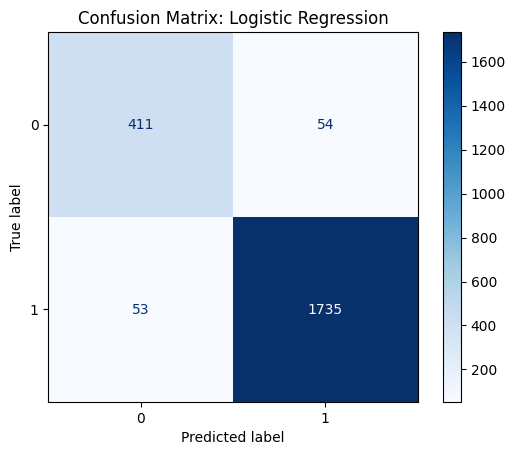
\includegraphics[width=0.45\textwidth]{images/cm_lr.png}
    \captionsetup{hypcap=false}
    \captionof{figure}{ماتریس درهم‌ریختگی مدل رگرسیون لجستیک; نرخ خطای بسیار پایین در شناسایی فایل‌های مخرب.}
    \label{fig:cm_lr}
\end{center}
}

\field{ مدل نایو بیز گوسی (\lr{Gaussian Naive Bayes})}{
در این فاز، مدل دسته‌بند بیز ساده (\lr{GaussianNB}) روی همان داده‌های مقیاس‌شده اعمال گردید. معیار عملکردی این مدل افت شدیدی را تجربه کرد و \textbf{دقت آن به حدود $68\%$} کاهش یافت.

\vspace{0.4cm}
\begin{center}
    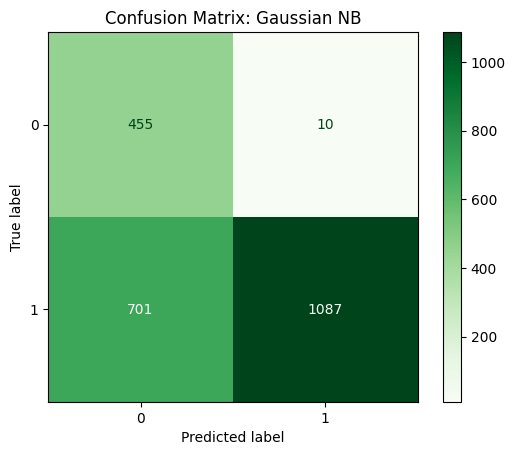
\includegraphics[width=0.45\textwidth]{images/cm_gnb.png}
    \captionsetup{hypcap=false}
    \captionof{figure}{ماتریس درهم‌ریختگی مدل نایو بیز; ناتوانی آشکار مدل در فیلتر کردن فایل‌های مخرب.}
    \label{fig:cm_gnb}
\end{center}
}

\field{ تحلیل و مقایسه عملکرد دو مدل بر اساس ماتریس درهم‌ریختگی}{
با تحلیل و مقایسه ماتریس‌های درهم‌ریختگی فوق، \textbf{مدل رگرسیون لجستیک عملکردی به مراتب برتر و پایدارتر} نشان می‌دهد. دلایل این برتری ملموس عبارتند از:
\begin{itemize}
    \item \textbf{کنترل فاجعه‌ی منفی کاذب (\lr{False Negative}):} در مسائل امنیت سایبری و بدافزار، ورود یک بدافزار به سیستم (منفی کاذب) بسیار خطرناک‌تر از مسدود شدن اشتباه یک فایل امن (مثبت کاذب) است. مدل رگرسیون لجستیک تنها ۵۳ بدافزار را از دست داده، در حالی که نایو بیز ۷۰۱ بدافزار (یک فاجعه امنیتی) را به اشتباه امن تشخیص داده است.
    \item \textbf{تحلیل مثبت کاذب (\lr{False Positive}):} با اینکه نرخ مثبت کاذب نایو بیز کمی کمتر است ($10$ در برابر $54$)، اما در حضور خطای هولناک ستون بدافزارهای فرار کرده، این معیار کاملاً ارزش خود را از دست می‌دهد.
    \item \textbf{علت ریاضی شکست نایو بیز:} الگوریتم نایو بیز فرض را بر \textbf{استقلال کامل ویژگی‌ها} از یکدیگر می‌گذارد. در داده‌های مربوط به بدافزارها، ویژگی‌های ساختاری فایل شدیداً به هم وابسته و هم‌بسته هستند. رگرسیون لجستیک با یادگیری دقیق وزن روابط فیچرها، این فرض محدودکننده را ندارد و به خوبی مرز تصمیم‌گیری را پیدا می‌کند.
\end{itemize}
}

\end{stepbox}